% Autor: Betti Oesterholz
% erstellt: 15.05.2011
% This is the handout for the Fib project.
%
% Copyright (c) 2011 Betti Oesterholz
%
% Permission is granted to copy, distribute and/or modify this document
% under the terms of the GNU Free Documentation License, Version 1.2 or
% any later version published by the Free Software Foundation;
% with no Invariant Sections, no Front-Cover Texts, and no Back-Cover Texts.
%
% A copy of the license is included in the file ``fdl.tex'' .
%


\documentclass[10pt,a4paper]{article}
\pagestyle{empty} %keine Seitennummerierung
\usepackage{a4wide} % besser den Platz nutzen (kleinere R"ander)
%\usepackage{ngerman} % Silbentrennung nach neuer Rechtschreibung
\usepackage[T1]{fontenc} % Type 1 Schriften
\usepackage{times} % Da die Standard-LaTeX-Schrift bei mir mit Acrobat nicht funkt.
\usepackage[ansinew]{inputenc} % Verwendung von Umlauten
%\usepackage{scrpage2} % Seitenformat
%\usepackage{titletoc}
%\usepackage{titlesec}
\usepackage{listings} % Programm-Listing
%\usepackage [usetoc]{titleref} 
\usepackage{graphicx} % Einbindung von Graphiken
\usepackage{url} % URLs durch \url{}
%\usepackage{bibgerm} % deutsche Bibliographie
%\usepackage{txfonts}%Paket fr das nat Symbol
\usepackage{multicol}
%\usepackage{makeidx}%for the index
%\usepackage{longtable}
%\usepackage{amsmath}%mathematikumgebung {equation*} usw.
\usepackage{picinpar}%Textumflossene Bilder

% Seitenstil festlegen
%\pagestyle{useheadings}%or: headings

% naehste vier Zeilen: Format des Inhaltsverzeichnisses
%\titlespacing{\section}{0pt}{5cm}{5cm}%spacing by sections {in front}{above}{below}
%\dottedcontents{section}[1.5em]{\addvspace{1.0em}}{1.3em}{0.7pc}
%\dottedcontents{subsection}[3.8em]{}{2.2em}{0.7pc}
%\dottedcontents{subsubsection}[7.0em]{}{3.1em}{0.7pc}

%\setcounter{secnumdepth}{4}%%nummerierung der Unterabschnitte bis Tiefe


%%%%%%%%%%%%%%%%%%%%%%%%%%%%%%%%%%%%%%%%%%%%%%%%%%%%%%%%%%%%%%%%%%%%%%%%%%%%%%%%%%%%%%%
% Beginn des Dokuments
%\makeindex

\begin{document}

%\renewcommand{\sectionmark}[1]{\markboth{#1}{}}
%\pagenumbering {Roman}
%\automark{section}
%\pagestyle{scrheadings} % individ. Seitenlayout
%\setheadsepline{0.4pt}
%\ihead{} % Titelzeile innen
%\ohead{} % Titelzeile aussen
%\chead{\slshape \headmark}  % Titelzeile mitte
%\cfoot{\thepage} % Fusszeile mitte

% braucht man ein Inhaltsverzeichnis, so sind die naehsten drei Zeilen auszukommentieren
%\setcounter{tocdepth}{3}
%\tableofcontents
%\clearpage

% Vorschlag fuer Titelzeile:
% Bei umfangreicheren Dokumenten
%\ihead{\slshape \headmark } % Darstellung von Sectionnummer und -name
%\ohead{}
%\chead{}


%\pagenumbering{arabic}


\ \vspace{-2.5cm}
\begin{center}
	\LARGE\bf The Fib multimedia system\\
\end{center}

\bigskip\noindent
The Fib multimedia system can be used to encode and store multimedia data (such as images or movies).
It is characterized by its universality and diversity.
\textbf{In this sense, the Fib multimedia system is based on diversity rather than specialization.}

This leads to a high complexity, as well as many possibilities for extensions and improvements. Therefore, the Fib system will be never truly complete, but always offer opportunities for further improvements.


%\section{Components}

The Fib system consists of several components. The most important are presented in the following.


\section{The Fib language}

\begin{window}[0,r,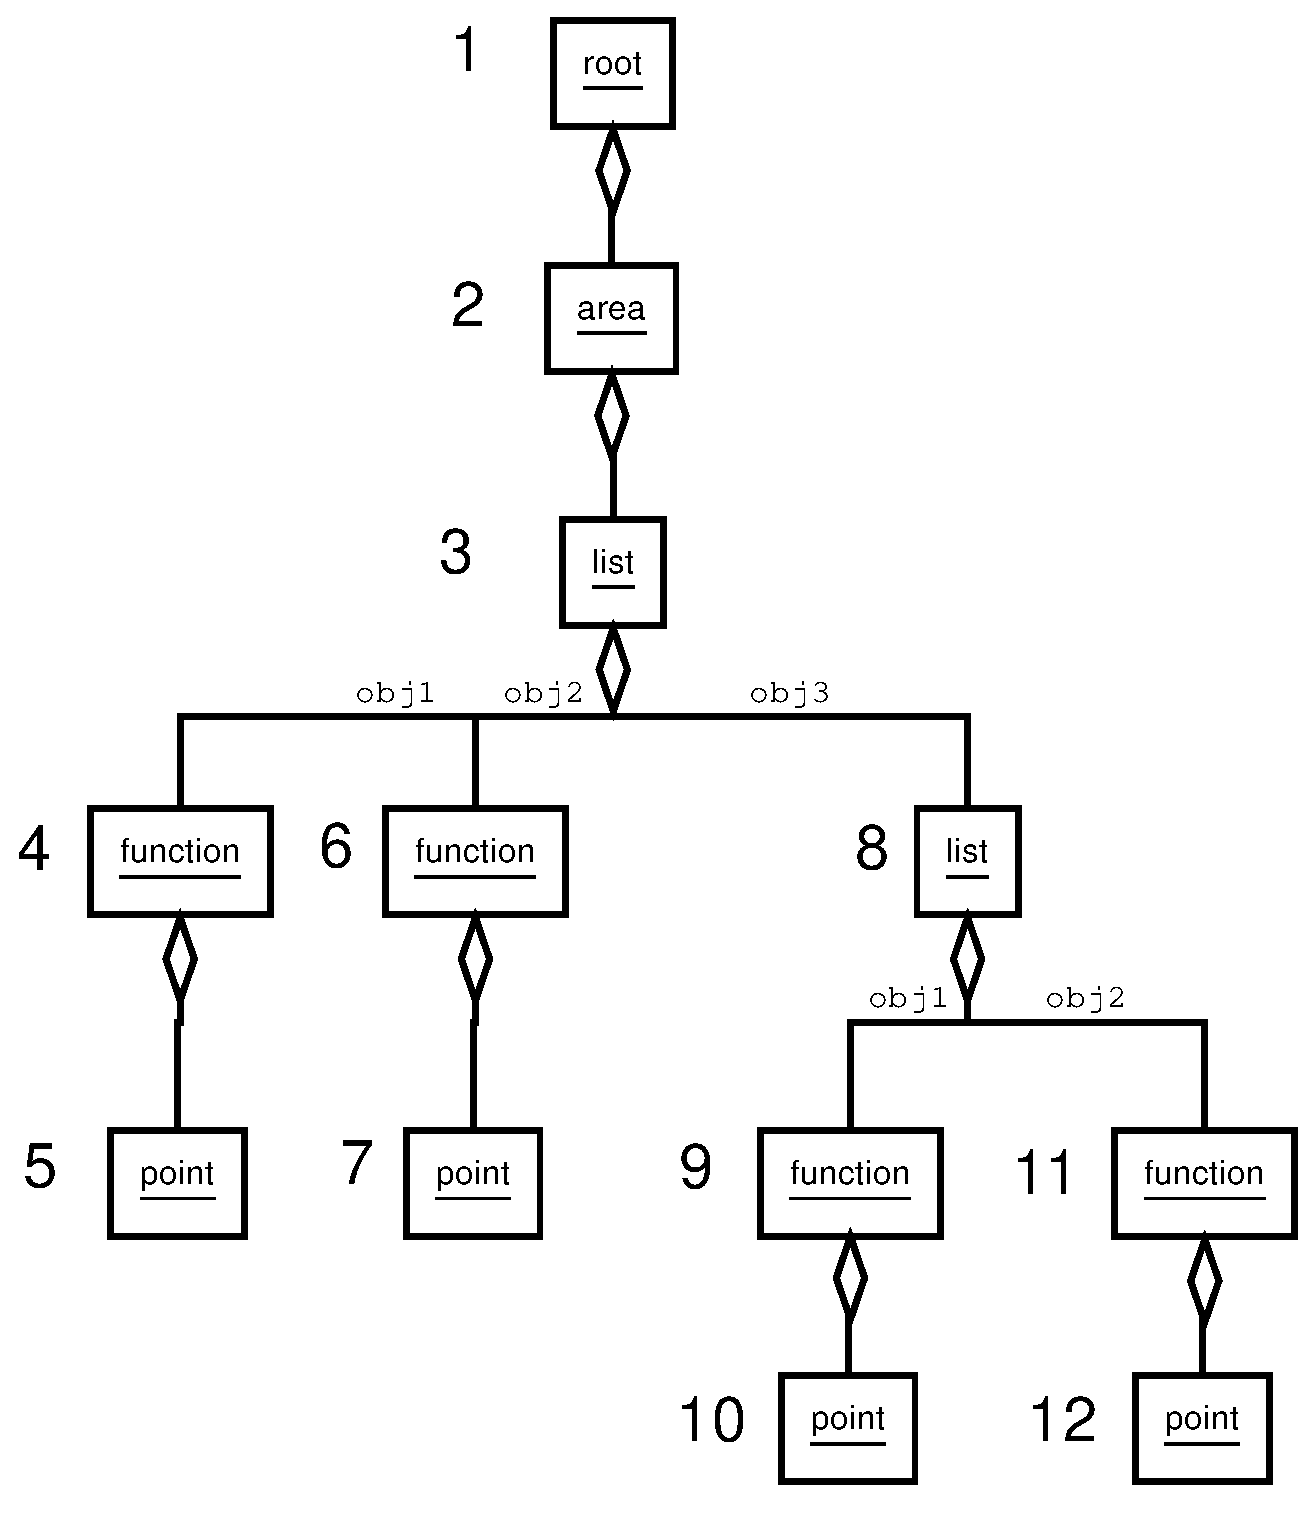
\includegraphics[scale=0.2]{./pictures/order_elements.eps},{}]
\noindent
The Fib multimedia format (Fib language) is used to store multimedia information in a structured, functional and hierarchical form. The structure of the Fib multimedia format supports the object view of things. The Fib format is very powerful, since expressions can be combined and nested (modular system).
\textbf{With Fib the question is not whether you can do something, but just how to do something.}
The memory cost of a multimedia object in Fib is much more dependent on its complexity as of its size (in terms of expansion in the dimensions, for example, the number of points in images), as in conventional multimedia formats.

The only restriction on the multimedia data, that can be displayed in the Fib format, is, that they can be represented as properties of points of a finite, euclidean and discrete (there are smallest units) space. Therefore, not only images and sounds can be stored with Fib, but for example also smells and how soft something is. Also objects and subobjects can be commented.
\end{window}

The basic framework for the Fib multimedia data is a tree. The leaves are endpoints, that are used for displaying respectively assignments to points or multimedia subobjects. In the branches and the alignment of these, which are, for example, on the leftmost, the display parameters or properties of the leaves are encoded, for example how often they are shown and with which color.


\section{The genetic algorithm}

\begin{window}[0,l,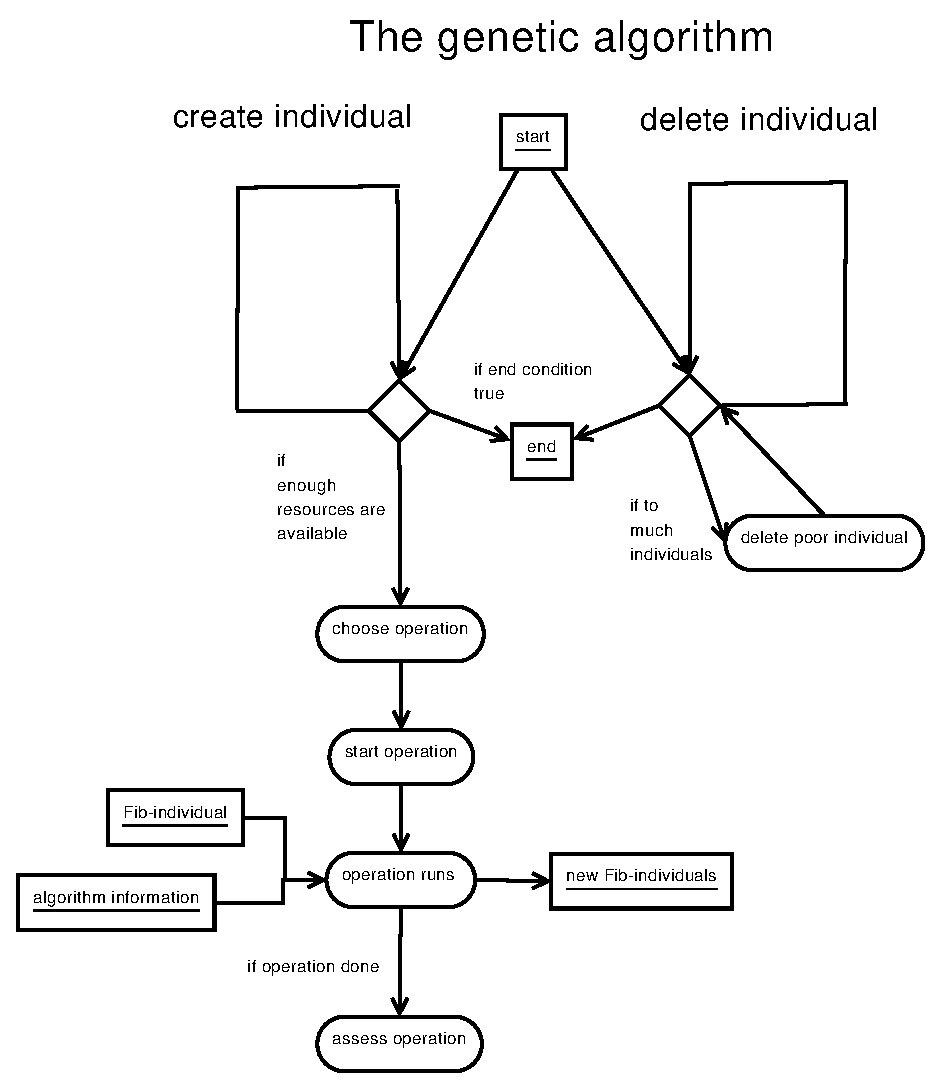
\includegraphics[scale=0.3]{./pictures/algorithmus.eps},{}]
\noindent
The second important component of the Fib system is the genetic algorithm for encoding and compressing of Fib multimedia objects. The great advantage of it is, that the encoding and compression is not bound by a particular algorithm, but that the actual encoding and compression algorithms are integrated into the genetic algorithm as operators, which can be easily added and modified. This makes it easy to introduce new encoding and compression ideas and apply a variety of these on a multimedia object.

In this sense, the genetic algorithm for Fib is a trans ingenious algorithm, that is designed to extract the ideas of people to encode multimedia data from their heads and then transport / collected them into a pool. Thus, these ideas / algorithms can accomplish more than they could individually.
\end{window}
The algorithm can thus combine more intelligence than one human (or a small group) can produce.


\section{Converters}

The converter programs for Fib are used to translate from other multimedia formats into the Fib format and vice versa. In this translation, some improvements of the target multimedia data are possible.


\end{document}







